\documentclass{article}

% Language setting
% Replace `english' with e.g. `spanish' to change the document language
\usepackage[english]{babel}
\usepackage{booktabs}
% Set page size and margins
% Replace `letterpaper' with `a4paper' for UK/EU standard size
\usepackage[letterpaper,top=2cm,bottom=2cm,left=3cm,right=3cm,marginparwidth=1.75cm]{geometry}
\usepackage{float}
\usepackage{adjustbox}
% Useful packages
\usepackage{amsmath}
\usepackage{graphicx}
\usepackage[colorlinks=true, allcolors=blue]{hyperref}
\usepackage{setspace}
\usepackage{rotating}
\usepackage{booktabs}
\usepackage{siunitx}
\usepackage{makecell}
\doublespacing % sets double spacinging

\title{ACARR Estimation, Conjecture and Problems on Our Study}
\author{Wen XU}
\date{2023-08-26}

\begin{document}
	\maketitle
	
	\section{Introduction}
	\begin{enumerate}
		
		\item
		In this file, I document the estimation of asymmetric conditional auto-regression of range (ACARR) model and several concerns of mine relating to this research.
		\item
		Following Chou (2006), the daily range estimator is decomposed into upward range and downward range. In the same spirit, we decompose the temperature spread into upward temperature spread  and  downward temperature spread. Specifically,
		
		
		\begin{subequations}
			\begin{equation}\label{t1}
				TS_{t}= H_t- L_t 
			\end{equation}
			\begin{equation}\label{t2}
				UTS_{t}= H_t- T_{t-1}
			\end{equation}
			\begin{equation}\label{t3}
				DTS_{t}= T_{t-1}- L_{t}
			\end{equation}
		\end{subequations}
		where $H_{t}$ denotes the highest temperatures at time t, where $L_{t}$ denotes the lowest temperatures at time t. $\log T_{t-1}$ denotes the average temperature at time $t-1$.
		
		\item The ACARR(p,q) model for the upward range is then estimated through
		
		\begin{subequations}
			\begin{equation}\label{t1}
				UTS_t= \lambda^u_t\epsilon_t\\
			\end{equation}
			\begin{equation}\label{t2}
				\lambda^u_t= \omega + \sum_{i=1}^{p}\alpha_{i}UTS_{t-{i}} + \sum_{i=1}^{q}\beta_{i}\lambda^u_{t-i}    
			\end{equation}
		\end{subequations}
		
		where $\lambda_{t}$ denotes the conditional mean of range at time {t}, and $\epsilon_{t}$ denotes the standardized residual at time t which assumes to follow a target distribution with unit mean. The ACARR model for the downward range works in the same manner. 
	\end{enumerate}
	
	\section{Estimation Procedure}
	
	
	I aware that it is not suitable for asking a professor to help me check with code. However, to make sure what i did is correct and make more sense for the following conjecture part, I attach the function part of CARR model. [The ACARR model is estimated with the same manner with CARR model but only changes the variables into the function]. During my estimation process, I utilize the normal distribution to maximize the targeted logliklihood function. Then, I select the best lag by using Bayesian Information Criteria (BIC).  The results of ACARR models are summarized at table 1-4.
	
	~\\
	
	\begin{figure}[H]
		
		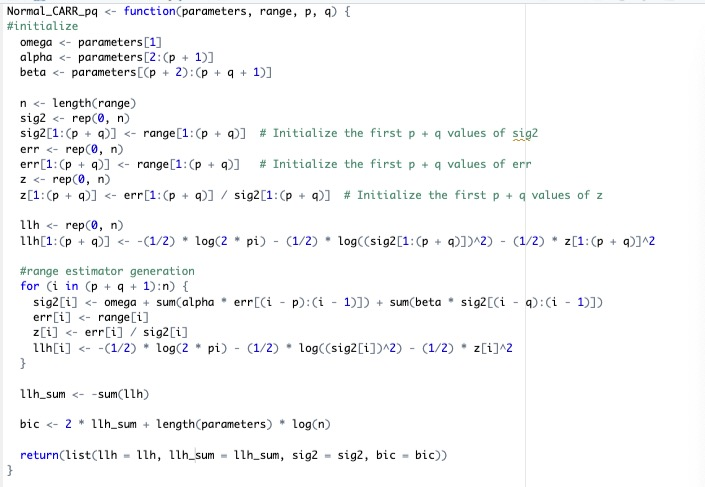
\includegraphics[width=1.2\textwidth, height=15cm]{/Applications/R/Weather_US/WechatIMG114.jpeg}
		
	\end{figure}
	\pagebreak
	
	
	
	
	\pagebreak
	
	\section{Conjecture and Problem}
	
	During my estimation process, i have found several problems.
	\begin{enumerate}
		\item Raw Data, Logged: ~\\
		From previous reports, we can clearly see that the temperature data is totally different from financial data. The significant characteristic of it is that the temperature can be negative and have strong seasonality. Therefore, how to solve these issues and how can we transform the data into the part we are familiar with becomes our first task. In terms of negative issues, I discussed with my supervisors and proposed to use the Kelvin to indicate the temperature and calculate the temperature range. However, we should work on the raw temperature data or the transformed temperature data is the part I still cannot figure out.  To the point of me, I am not really convinced by using the raw data temperature. My concerns are as follows. 1: Our target is the forecast of range, which has to be positive.  Using the raw data may not be proper. For example, when the linear-based-heterogenous autoregression model (HAR) is employed, it still has a chance to generate a negative value. 2:  I believe Kelvin still have to be used to make sure the temperature is positive. In terms of the zero range issue, I am not fully persuaded because the adding term is only 273.15 which is not a large number. [Note that: The price of the Japanese stock index, Nikkei 225, is nearly 30,000 which is still available to calculate returns and range] 
		
		\item Using the $T_{t-1}$ as the base: ~\\
		The second issue occurs at the asymmetric range estimation. See the data generating process of the $UTS_{t}$ and $DTS_{t}$ in Equation 1.  The calculation is totally different from Chou (2006). We can promise the asymmetric range at time t is positive, however, we cannot promise the asymmetric range across the period is positive. The same for the temperature data. There are over 30 of 10,000 observations that are negative value in both $UTS_{t}$ and $DTS_{t}$, but the good news is both of them are stationary. [I do also try to use the difference between variables at the same date to conduct estimation. The result can be given upon request. Note that, if we use the difference the same to conduct estimation, we should mainly be concerned the seasonal trend. Namely, the difference between high in summer must be different from winter in some places].
		
		\item CARR model: ~\\
		Following the previous issue, when the temperature range is negative, we can see that the CARR model is still can be estimated. However, it actually does not make sense due to the volatility cannot be negative. I believe the reason why it can be estimated is that its structure is different from GARCH. For the financial data and asymmetric range in Chou (2006), the daily range and the conditional mean of the range are restricted to be positive and these provide the advantage that we can use the GARCH model package to obtain the results by only substituting returns into squared root of range. However, when the negative value occurs and the GARCH package is no longer useful, it actually still works on writing the MLE function directly. [Wu proposes to use absolute value to overcome this issue. In my opinion, it disobeys the nature of the ACARR model. Namely, the spirit of Chou (2006) is to generate the downard range and upward range, then sum them so as to improve the forecast of range. However, when the absolute value is taken, this equality does not work any longer. ]
		
		\item Some small points:~\\
		(1) Seasonality issue: From previous literature, such as Campell and Diebold (2005), the seasonality issue is obtained by Fourier Transformation. The trend is also modelled as a function of time. Wu proposes to use ARIMA to overcome these issues. From my side, it is doable but we still try to eliminate these effects so as to obtain the stationary process rather than the risk of temperature. 
		~\\
		
		(2) Practical Implications: Except for the technical issue, one of the most important thing is that we need to find out some implications of our proposed model. For the financial data, we could say a more accurate forecast of the range potentially could affect the value at risk. However, for the temperature, what we should be concerned? Most of the literature focus on weather Derivative, such as Campell and Diebold (2005). However, it requires a strong math background and is inefficient. Engle (2020) documents that there are two types of climate risk. The first is what we are trying to model and forecast. He named this after "physical climate risk". The second is regulator interventions. The impact of this was obtained from the media posts, investors' concerns, ESG, and many others. Stock market investors are prone to focus on the second one rather than the first. 	From my intuitive thinking, what we can try to explore is the equity risk premium and the potential cointegration. The most related to the physical risk of climate would be real estate (sea level), electricity price, and energy price. However, it is still at the brainstorming stage. More details need to be thought twice.
		~\\
		(3) Finally, why asymmetric range is imporant may be also the important thing to answer.
	\end{enumerate}	
	
	\section{Reference}	
	1. Campbell, S. D., \& Diebold, F. X. (2005). Weather forecasting for weather derivatives. Journal of the American Statistical Association, 100(469), pp. 6-16.
	~\\
	2. Chou, R.Y., 2006. Modeling the asymmetry of stock movements using price ranges. In Econometric Analysis of Financial and Economic Time Series, pp. 231-257. 
	~\\	
	3. Engle, R.F., Giglio, S., Kelly, B., Lee, H. and Stroebel, J., 2020. Hedging climate change news. The Review of Financial Studies, 33(3), pp.1184-1216.
	\begin{sidewaystable}[htbp]
		\centering
		\caption{DTS Estimation with $\omega$ = 0.01, $\alpha$ = 0.1, $\beta$ = 0.2 as initial values}
		\begin{tabular}{cccccccccccccc}
			\toprule
			
			& Atlanta & Boston & Burbank & Chicago & Cincinnati & Dallas & Houston & Las Vegas & Minneapolis & New York & Philadelphia & Portland & Sacramento \\
			\midrule
			$\omega$ & 0.400 & 0.400 & 0.400 & 0.400 & 0.400 & 0.267 & 0.141 & 0.400 & 0.400 & 0.400 & 0.400 & 0.400 & 0.400 \\
			& [0.143] & [0.233] & [0.521] & [0.103] & [0.176] & [0.089] & [0.079] & [0.214] & [0.239] & [0.233] & [0.246] & [0.131] & [0.219] \\
			$\alpha_{1}$  & 0.185 &	0.130 &	0.439 &	0.089 	&0.067 	&0.092 	&0.140 &	0.139 &	0.037 	&0.100 	&0.121 	&0.300 &	0.223 \\
			& [0.022] & [0.027] & [0.080] & [0.017] & [0.013] & [0.092] & [0.038] & [0.014] & [0.012] & [0.029] & [0.029] & [0.034] & [0.043] \\
			$\beta_{1}$  & 0.445 &	0.300 	&0.274 &	0.250 &	0.274 &	0.364 &	0.523 &	0.833 &	0.730 &	0.387 &	0.523 &	0.214 &	0.477  \\
			&[0.124] 	&[0.211] &[0.199]& 	[0.161]	&[0.227]&[0.167]&[0.085]&[0.051]&[0.068]&[0.257]&[0.189]&[0.095]&[0.187] \\
			$\beta_{2}$ &0.334 &	0.538 &	0.047 &	0.623 &	0.617 &	0.527 &	0.335 &&0.194 &	0.478 &0.320 & 0.104 &0.267  \\
			& [0.114] &	[0.166] &	[0.251] &	[0.100] &	[0.150] &	[0.126] &	[0.083] &&	[0.082] &	[0.223] &	[0.189] &	[0.116] 	&[0.210]  \\
			$\beta_{3}$ & $<$0.001 	&$<$0.001 	&0.216 &	$<$0.001 &	$<$0.001 &	$<$0.001 &	$<$0.001 &	&&	$<$0.001 &	$<$0.001 &	0.106 &	 \\
			& [0.126] &	[0.220] &	[0.203 ]&	[0.165]&	[0.234]&	[0.164]&	[0.093]&	&&[0.269] &	[0.216]& 	[0.122] &	   \\
			$\beta_{4}$ & &   &   &   &   &  & &   &   &   &   & 0.080 &   \\
			&  &   &   &   &   &  &  &   &   &   &   & [0.121] &   \\
			$\beta_{5}$ &  &   &   &   &   &  &  &   &   &   &   & 0.161&   \\
			& &   &   &   &   & &  &   &   &   &   & [0.115] &   \\
			\bottomrule
		\end{tabular}
	\end{sidewaystable}
	
	
	
	
	
	\begin{sidewaystable}[htbp]
		\centering
		\caption{UTS Estimation with $\omega = 0.01$, $\alpha = 0.1$, $\beta = 0.2$ as initial values}
		\begin{tabular}{cccccccccccccc}
			\toprule
			& Atlanta & Boston & Burbank & Chicago & Cincinnati & Dallas & Houston & Las Vegas & Minneapolis & New York & Philadelphia & Portland & Sacramento \\
			\midrule
			$\omega$ & 0.400 & 0.400 & 0.400 & 0.400 & 0.400 & 0.370 & 0.400 & 0.400 & 0.400 & 0.400 & 0.400 & 0.400 & 0.400 \\
			& [0.345] & [0.268] & [0.737] & [0.049] & [0.186] & [0.217] & [0.306] & [0.618] & [0.239] & [0.243] & [0.307] & [0.152] & [0.389] \\
			$\alpha_{1}$  & $<$0.001  & $<$0.001  & 0.639 & 0.331 & 0.166 & $<$ 0.001  & $<$ 0.001  & 0.304 & $<$ 0.001  & 0.179 & $<$ 0.001  & 0.414 & 0.516 \\
			& [0.116] & [0.086] & [0.075] & [0.003] & [0.019] & [0.047] & [0.049] & [0.061] & [0.071] & [0.019] & [0.079] & [0.032] & [0.056] \\
			$\beta_{1}$   & $<$ 0.001  & 0.185 & 0.168 & 0.264 & 0.303 & 0.168 & $<$ 0.001  & 0.260 & 0.144 & 0.294 & 0.190 & 0.227 & 0.229 \\
			& [0.183] & [0.025] & [0.113] & [0.029] & [0.123] & [0.017] & [0.038] & [0.205] & [0.013] & [0.127] & [0.019] & [0.079] & [0.150] \\
			$\beta_{2}$   & $<$0.001  & 0.283 & 0.059 & 0.062 & 0.329 & 0.316 & 0.190 & 0.148 & 0.224 & 0.261 & 0.300 & 0.053 & 0.113 \\
			& [0.187] & [0.182] & [0.157] & [0.032] & [0.112] & [0.133] & [0.021] & [0.232] & [0.184] & [0.131] & [0.171] & [0.085] & [0.170] \\
			$\beta_{3}$   & $<$ 0.001 & 0.194 & 0.120 & 0.340 & 0.172 & 0.155 & 0.400 & 0.255 & 0.230 & 0.235 & 0.222 & 0.209 & 0.119 \\
			& [0.141] & [0.132] & [0.149] & [0.018] & [0.109] & [0.133] & [0.100] & [0.214] & [0.181] & [0.136] & [0.136] & [0.080] & [0.175] \\
			$\beta_{4}$   & 0.224 & & & & & 0.322 & 0.303 & & & & & 0.137 & \\
			& 0.025 & & & & & 0.116 & 0.111 & & & & & 0.144 & \\
			$\beta_{5}$   & 0.258 & & & & & 0.011 & 0.070 & & & & & [0.121] & \\
			& [0.212] & & & & & [0.128] & [0.207] & & & & & [0.118] & \\
			\bottomrule
		\end{tabular}
	\end{sidewaystable}
	
	
	
	\begin{sidewaystable}[htbp]
		\centering
		\caption{DTS Estimation with $\omega$ = 0.01, $\alpha$ = 0.1, $\beta$ = 0.2 as initial values}
		\begin{tabular}{cccccccccccccc}
			\toprule
			& Atlanta & Boston & Burbank & Chicago & Cincinnati & Dallas & Houston & Las Vegas & Minneapolis & New York & Philadelphia & Portland & Sacramento \\
			\midrule
			$\omega$ & 0.400 & 0.400 & 0.400 & 0.400 & 0.400 & 0.370 & 0.400 & 0.400 & 0.400 & 0.400 & 0.400 & 0.400 & 0.400\\
			& [0.345] & [0.268] & [0.737] & [0.049] & [0.186] & [0.217] & [0.306] & [0.618] & [0.239] & [0.243] & [0.307] & [0.152] & [0.389] \\
			$\alpha_{1}$  & $<$0.001  & $<$0.001  & 0.639 & 0.331 & 0.166 & $<$ 0.001  & $<$ 0.001  & 0.304 & $<$ 0.001  & 0.179 & $<$ 0.001  & 0.414 & 0.516 \\
			& [0.116] & [0.086] & [0.075] & [0.003] & [0.019] & [0.047] & [0.049] & [0.061] & [0.071] & [0.019] & [0.079] & [0.032] & [0.056] \\
			$\beta_{1}$   & $<$ 0.001  & 0.185 & 0.168 & 0.264 & 0.303 & 0.168 & $<$ 0.001  & 0.260 & 0.144 & 0.294 & 0.190 & 0.227 & 0.229 \\
			& [0.183] & [0.025] & [0.113] & [0.029] & [0.123] & [0.017] & [0.038] & [0.205] & [0.013] & [0.127] & [0.019] & [0.079] & [0.150] \\
			$\beta_{2}$   & $<$ 0.001  & 0.283 & 0.059 & 0.062 & 0.329 & 0.316 & 0.190 & 0.148 & 0.224 & 0.261 & 0.300 & 0.053 & 0.113 \\
			& [0.187] & [0.182] & [0.157] & [0.032] & [0.112] & [0.133] & [0.021] & [0.232] & [0.184] & [0.131] & [0.171] & [0.085] & [0.170] \\
			$\beta_{3}$   & $<$ 0.001 & 0.194 & 0.120 & 0.340 & 0.172 & 0.155 & 0.400 & 0.255 & 0.230 & 0.235 & 0.222 & 0.209 & 0.119 \\
			& [0.141] & [0.132] & [0.149] & [0.018] & [0.109] & [0.133] & [0.100] & [0.214] & [0.181] & [0.136] & [0.136] & [0.080] & [0.175] \\
			$\beta_{4}$   & 0.224 & & & & & 0.322 & 0.303 & & & & & 0.137 & \\
			& 0.025 & & & & & 0.116 & 0.111 & & & & & 0.144 & \\
			$\beta_{5}$   & 0.258 & & & & & 0.011 & 0.070 & & & & & [0.121] & \\
			& [0.212] & & & & & [0.128] & [0.207] & & & & & [0.118] & \\
			\bottomrule
		\end{tabular}
	\end{sidewaystable}
	
	
	
	\begin{sidewaystable}[htbp]
		\centering
		\caption{UTS Estimation with $\omega$ = 0.3, $\alpha$ = 0.01, $\beta$ = 0.02 as initial values}
		\begin{tabular}{cccccccccccccc}
			\toprule
			& Atlanta & Boston & Burbank & Chicago & Cincinnati & Dallas & Houston & Las Vegas & Minneapolis & New York & Philadelphia & Portland & Sacramento \\
			\midrule
			$\omega$ & 0.400 & 0.400 & 0.400 & 0.400 & 0.400 & 0.370 & 0.400 & 0.400 & 0.400 & 0.400 & 0.400 & 0.400 &0.400\\
			& [$0.345$] & [$0.268$] & [$0.737$] & [$0.049$] & [$0.186$] & [$0.217$] & [$0.306$] & [$0.618$] & [$0.239$] & [$0.243$] & [$0.307$] & [$0.152$] & [$0.389$] \\
			$\alpha_{1}$  & $<$0.001 & $<$0.001 & 0.639 & 0.331 & 0.166 & $<$0.001 & $<$0.001 & 0.304 & $<$0.001 & 0.179 & $<$0.001 & 0.414 & 0.516 \\
			& [0.116] & [0.086] & [0.075] & [0.003] & [0.019] & [0.047] & [0.049] & [0.061] & [0.071] & [0.019] & [0.079] & [0.032] & [0.056] \\
			$\beta_{1}$ & $<$0.001 & 0.185 & 0.168 & 0.264 & 0.303 & 0.168 & $<$0.001 & 0.260 & 0.144 & 0.294 & 0.190 & 0.227 & 0.229 \\
			& [0.183] & [0.025] & [0.113] & [0.029] & [0.123] & [0.017] & [0.038] & [0.205] & [0.013] & [0.127] & [0.019] & [0.079] & [0.150] \\
			$\beta_{2}$ & $<$0.001 & 0.283 & 0.059 & 0.062 & 0.329 & 0.316 & 0.190 & 0.148 & 0.224 & 0.261 & 0.300 & 0.053 & 0.113 \\
			& [0.187] & [0.182] & [0.157] & [0.032] & [0.112] & [0.133] & [0.021] & [0.232] & [0.184] & [0.131] & [0.171] & [0.085] & [0.170] \\
			$\beta_{3}$  & $<$0.001 & 0.194 & 0.120 & 0.340 & 0.172 & 0.155 & 0.400 & 0.255 & 0.230 & 0.235 & 0.222 & 0.209 & 0.119 \\
			& [0.141] & [0.132] & [0.149] & [0.018] & [0.109] & [0.133] & [0.100] & [0.214] & [0.181] & [0.136] & [0.136] & [0.080] & [0.175] \\
			$\beta_{4}$  & 0.224] & & & & & 0.322 & 0.303 & & & & & 0.137 & \\
			& [0.025] & & & & & [0.116] & [0.111] & & & & & [0.144] & \\
			$\beta_{5}$  & 0.258 & & & & & 0.011 & 0.070 & & & & & 0.121 & \\
			& [0.212] & & & & & [0.128] & [0.207] & & & & & [0.118] & \\
			
			\bottomrule
		\end{tabular}
	\end{sidewaystable}
	
	
	
\end{document}


